\documentclass[tikz]{standalone}
\usepackage{pgfplots}
\pgfplotsset{compat=1.15}
\usepackage{mathrsfs}
\usetikzlibrary{arrows,calc}
\usepackage{tkz-euclide}

\pagestyle{empty}

\definecolor{AngleClr}{rgb}{0,0.39215686274509803,0}
\definecolor{ShapeClr}{rgb}{0.6,0.2,0}
\definecolor{ParacircleClr}{RGB}{217,185,7}
\definecolor{BlueSqr}{RGB}{5,81,163}

\begin{document}

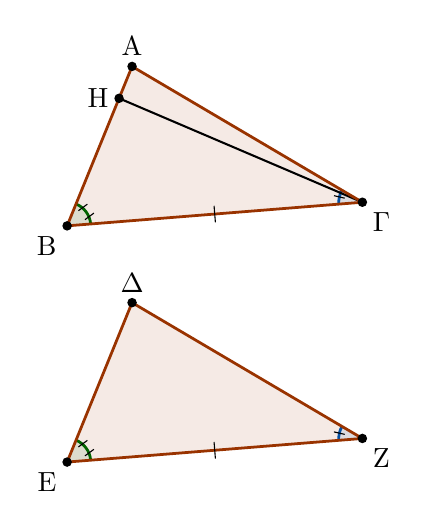
\begin{tikzpicture}[scale=.75]
\tkzSetUpLine[line width=1pt,color=black]
\tkzSetUpPoint[fill=black]

\tkzDefPoints{0/0/B,1.1/2.7/A,5/0.4/C}
\tkzDefPoints{0/-4/E,1.1/-1.3/D,5/-3.6/Z}

\tkzDefPointOnLine[pos=0.2](A,B)\tkzGetPoint{H}

\tkzFillPolygon[fill=ShapeClr,fill opacity=0.1](A,B,C)
\tkzFillPolygon[fill=ShapeClr,fill opacity=0.1](D,E,Z)

\tkzFillAngle[fill=AngleClr,size=.4,fill opacity=0.1](C,B,A)
\tkzMarkAngle[mark=||,mksize=2,line width=1pt,color=AngleClr,size=.4](C,B,A)

\tkzFillAngle[fill=AngleClr,size=.4,fill opacity=0.1](Z,E,D)
\tkzMarkAngle[mark=||,mksize=2,line width=1pt,color=AngleClr,size=.4](Z,E,D)

\tkzFillAngle[fill=BlueSqr,size=.4,fill opacity=0.1](A,C,B)
\tkzMarkAngle[mark=|,mksize=2,line width=1pt,color=BlueSqr,size=.4](A,C,B)

\tkzFillAngle[fill=BlueSqr,size=.4,fill opacity=0.1](D,Z,E)
\tkzMarkAngle[mark=|,mksize=2,line width=1pt,color=BlueSqr,size=.4](D,Z,E)


\tkzDrawSegments[line width=0.75pt,color=black](C,H)

\tkzDrawPolygon[color=ShapeClr](A,B,C)
\tkzDrawPolygon[color=ShapeClr](D,E,Z)

\tkzDrawPoints[size=3](A,B,C,D,E,Z,H)

\tkzLabelPoint[above](A){$\rm A$}
\tkzLabelPoint[below left](B){$\rm B$}
\tkzLabelPoint[below right](C){$\rm \Gamma$}

\tkzLabelPoint[above](D){$\rm\Delta$}
\tkzLabelPoint[below left](E){$\rm E$}
\tkzLabelPoint[below right](Z){$\rm Z$}

\tkzLabelPoint[left](H){$\rm H$}

\tkzMarkSegments[mark=|,size=3](B,C E,Z)

\end{tikzpicture}

\end{document}
